\documentclass{article}
\usepackage[T1]{fontenc}
\usepackage[utf8]{inputenc}
\usepackage[ngerman]{babel}
\usepackage{fullpage}
\usepackage{tikz}
\usepackage{amsmath} 
\usepackage{amsfonts}
\usepackage{amssymb}
\usepackage{mathtools}
\setlength{\parindent}{0pt}
\pagestyle{empty}
\begin{document}
\section{Algebraischer Beweis H"ohensatz}

\begin{align*}
a^2 + b^2 &= c^2\\ 
h^2 + p^2 &= a^2\\
h^2 + q^2 &= b^2
\end{align*}

Ausserdem gilt \( p+q = c \) und quadriert:

\[ (p + q)^2 = c^2\]

Nach der ersten binomischen Formeln ist das:

\[ p^2 + 2pq + q^2 = c^2 \]

Das kann man jetzt fuer $c^2$ in der ersten Formel einsetzen und $a^2$ und $b^2$ mit der 2. und 3. Formel ersetzen:

\[ h^2 + p^2 + h^2 + q^2 = p^2 + 2pq + q^2 \]

Daraus folgt

\[ h^2=pq \]

\section{Algebraischer Beweis Kathetensatz}

Analog wie der Beweis zum H"ohensatz verl"auft auch dieser Beweis. Es gilt:

\[ a^2 = c^2-b^2=p^2+2pq+q^2-(q^2+h^2)=p^2+2pq+q^2-q^2\underbrace{-a^2+p^2}_{\mathclap{\text{da ja gilt: } h^2 + p^2 = a^2}}=2p^2+2pq-a^2 \]

vereinfacht folgt:

\[ 2a^2 = 2p(p + q) = 2pc \]

also 

\[ a^2 = pc \]

und analog folgt:

\[ b^2 = qc \]

\begin{figure}[h]
\centering
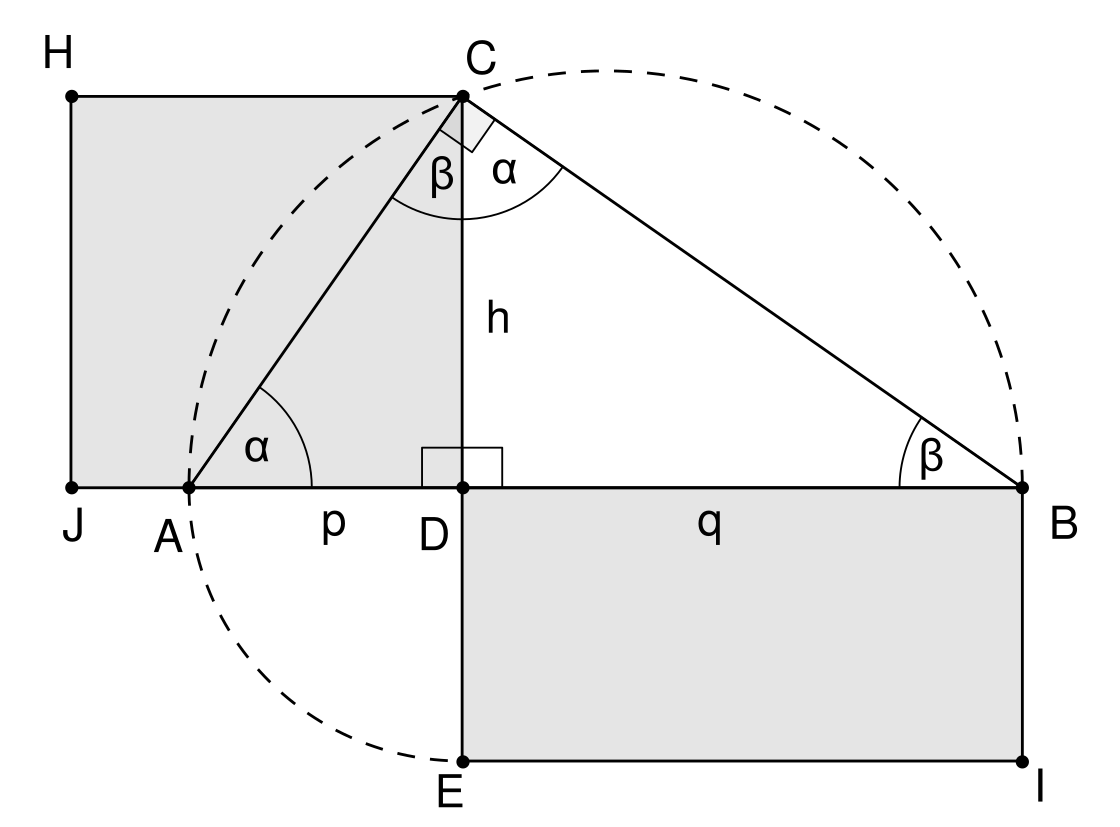
\includegraphics[width=0.35\textwidth]{Hoehensatz}
\end{figure}


\newpage
\begin{figure}[t]
\begin{tikzpicture}[scale=4]
\draw[fill=gray, fill opacity=0.2,rotate=23] (0,0) -- (1,0) -- (1,1) -- (0,1) -- cycle;
\end{tikzpicture}
\end{figure}
\end{document}